\documentclass{standalone}
\usepackage{tikz}
\usetikzlibrary{patterns, positioning}
\usepackage[sfdefault]{ClearSans} %% option 'sfdefault' activates Clear Sans as the default text font
\usepackage[T1]{fontenc}

\begin{document}
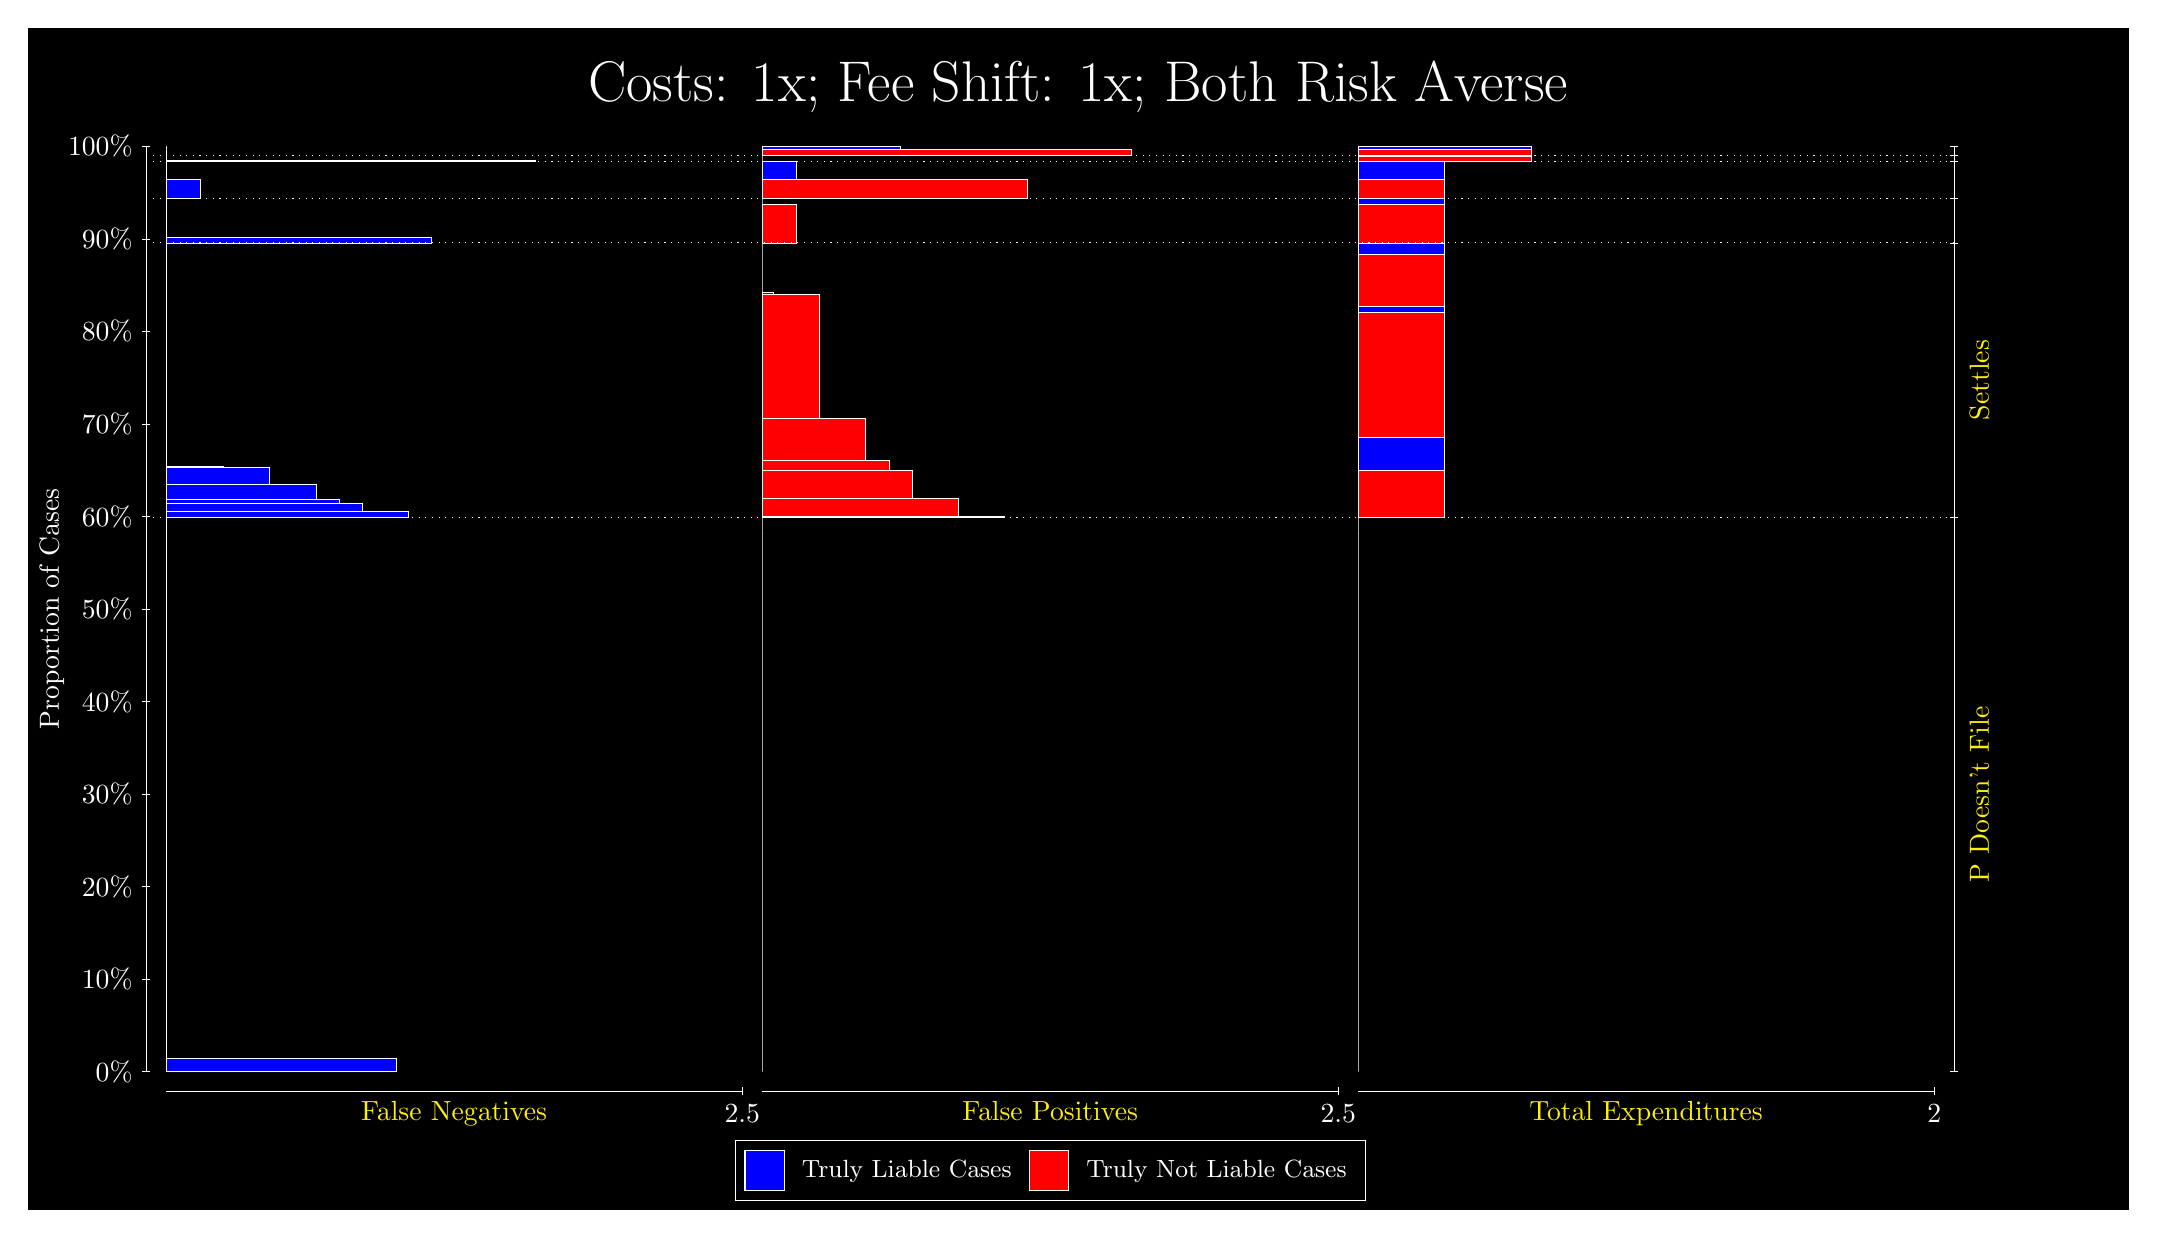
\begin{tikzpicture}
\draw[fill=black] (0,0) rectangle (26.667,15);
\draw[text=white] (0,13.5) rectangle (26.667,15) node[midway] {\huge Costs: 1x; Fee Shift: 1x; Both Risk Averse};
\draw[white, very thin] (1.5,1.75) -- (1.5,13.5);
\node[rotate=90, text=white, anchor=center] at (0.3, 7.625) {Proportion of Cases};
\draw[white, very thin] (1.45,1.75) -- (1.55,1.75);
\node[text=white, anchor=east] at (1.45, 1.75) {0\%};
\draw[white, very thin] (1.45,2.925) -- (1.55,2.925);
\node[text=white, anchor=east] at (1.45, 2.925) {10\%};
\draw[white, very thin] (1.45,4.1) -- (1.55,4.1);
\node[text=white, anchor=east] at (1.45, 4.1) {20\%};
\draw[white, very thin] (1.45,5.275) -- (1.55,5.275);
\node[text=white, anchor=east] at (1.45, 5.275) {30\%};
\draw[white, very thin] (1.45,6.45) -- (1.55,6.45);
\node[text=white, anchor=east] at (1.45, 6.45) {40\%};
\draw[white, very thin] (1.45,7.625) -- (1.55,7.625);
\node[text=white, anchor=east] at (1.45, 7.625) {50\%};
\draw[white, very thin] (1.45,8.8) -- (1.55,8.8);
\node[text=white, anchor=east] at (1.45, 8.8) {60\%};
\draw[white, very thin] (1.45,9.975) -- (1.55,9.975);
\node[text=white, anchor=east] at (1.45, 9.975) {70\%};
\draw[white, very thin] (1.45,11.15) -- (1.55,11.15);
\node[text=white, anchor=east] at (1.45, 11.15) {80\%};
\draw[white, very thin] (1.45,12.325) -- (1.55,12.325);
\node[text=white, anchor=east] at (1.45, 12.325) {90\%};
\draw[white, very thin] (1.45,13.5) -- (1.55,13.5);
\node[text=white, anchor=east] at (1.45, 13.5) {100\%};

\draw[white, very thin] (24.457,1.75) -- (24.457,13.5);
\draw[white, very thin] (24.407,1.75) -- (24.507,1.75);
\node[anchor=west] at (24.407, 1.75) {};
\draw[white, very thin] (24.407,8.7889) -- (24.507,8.7889);
\node[anchor=west] at (24.407, 8.7889) {};
\draw[white, very thin] (24.407,12.274) -- (24.507,12.274);
\node[anchor=west] at (24.407, 12.274) {};
\draw[white, very thin] (24.407,12.842) -- (24.507,12.842);
\node[anchor=west] at (24.407, 12.842) {};
\draw[white, very thin] (24.407,13.31) -- (24.507,13.31);
\node[anchor=west] at (24.407, 13.31) {};
\draw[white, very thin] (24.407,13.384) -- (24.507,13.384);
\node[anchor=west] at (24.407, 13.384) {};
\draw[white, very thin] (24.407,13.5) -- (24.507,13.5);
\node[anchor=west] at (24.407, 13.5) {};

\draw[white, very thin, fill=blue] (1.75,1.75) rectangle (4.6775,1.9166);
\draw[white, very thin, fill=red] (1.75,1.9166) rectangle (1.75,8.7889);
\draw[white, very thin, fill=blue] (1.75,8.7889) rectangle (4.8239,8.8697);
\draw[white, very thin, fill=blue] (1.75,8.8697) rectangle (4.2384,8.9722);
\draw[white, very thin, fill=blue] (1.75,8.9722) rectangle (3.9457,9.0154);
\draw[white, very thin, fill=blue] (1.75,9.0154) rectangle (3.6529,9.2039);
\draw[white, very thin, fill=blue] (1.75,9.2039) rectangle (3.0674,9.4181);
\draw[white, very thin, fill=blue] (1.75,9.4181) rectangle (2.4819,9.4426);
\draw[white, very thin, fill=red] (1.75,9.4426) rectangle (1.75,12.274);
\draw[white, very thin, fill=blue] (1.75,12.274) rectangle (5.1167,12.347);
\draw[white, very thin, fill=red] (1.75,12.347) rectangle (1.75,12.842);
\draw[white, very thin, fill=blue] (1.75,12.842) rectangle (2.1891,13.077);
\draw[white, very thin, fill=red] (1.75,13.077) rectangle (1.75,13.31);
\draw[white, very thin, fill=blue] (1.75,13.31) rectangle (6.4341,13.319);
\draw[white, very thin, fill=red] (1.75,13.319) rectangle (1.75,13.384);
\draw[white, very thin, fill=red] (1.75,13.384) rectangle (1.75,13.461);
\draw[white, very thin, fill=blue] (1.75,13.461) rectangle (1.75,13.5);
\draw[white, very thin, fill=red] (9.3189,1.75) rectangle (9.3189,8.6223);
\draw[white, very thin, fill=blue] (9.3189,8.6223) rectangle (9.3189,8.7889);
\draw[white, very thin, fill=red] (9.3189,8.7889) rectangle (12.393,8.8049);
\draw[white, very thin, fill=red] (9.3189,8.8049) rectangle (11.807,9.0332);
\draw[white, very thin, fill=red] (9.3189,9.0332) rectangle (11.222,9.3815);
\draw[white, very thin, fill=red] (9.3189,9.3815) rectangle (10.929,9.5178);
\draw[white, very thin, fill=red] (9.3189,9.5178) rectangle (10.636,10.042);
\draw[white, very thin, fill=red] (9.3189,10.042) rectangle (10.051,11.62);
\draw[white, very thin, fill=blue] (9.3189,11.62) rectangle (9.4652,11.645);
\draw[white, very thin, fill=blue] (9.3189,11.645) rectangle (9.3189,12.274);
\draw[white, very thin, fill=red] (9.3189,12.274) rectangle (9.758,12.769);
\draw[white, very thin, fill=blue] (9.3189,12.769) rectangle (9.3189,12.842);
\draw[white, very thin, fill=red] (9.3189,12.842) rectangle (12.686,13.076);
\draw[white, very thin, fill=blue] (9.3189,13.076) rectangle (9.758,13.31);
\draw[white, very thin, fill=red] (9.3189,13.31) rectangle (9.3189,13.375);
\draw[white, very thin, fill=blue] (9.3189,13.375) rectangle (9.3189,13.384);
\draw[white, very thin, fill=red] (9.3189,13.384) rectangle (14.003,13.461);
\draw[white, very thin, fill=blue] (9.3189,13.461) rectangle (11.075,13.5);
\draw[white, very thin, fill=red] (16.888,1.75) rectangle (16.888,8.6223);
\draw[white, very thin, fill=blue] (16.888,8.6223) rectangle (16.888,8.7889);
\draw[white, very thin, fill=red] (16.888,8.7889) rectangle (17.986,9.3815);
\draw[white, very thin, fill=blue] (16.888,9.3815) rectangle (17.986,9.8087);
\draw[white, very thin, fill=red] (16.888,9.8087) rectangle (17.986,11.387);
\draw[white, very thin, fill=blue] (16.888,11.387) rectangle (17.986,11.467);
\draw[white, very thin, fill=red] (16.888,11.467) rectangle (17.986,12.128);
\draw[white, very thin, fill=blue] (16.888,12.128) rectangle (17.986,12.274);
\draw[white, very thin, fill=red] (16.888,12.274) rectangle (17.986,12.769);
\draw[white, very thin, fill=blue] (16.888,12.769) rectangle (17.986,12.842);
\draw[white, very thin, fill=red] (16.888,12.842) rectangle (17.986,13.076);
\draw[white, very thin, fill=blue] (16.888,13.076) rectangle (17.986,13.31);
\draw[white, very thin, fill=red] (16.888,13.31) rectangle (19.083,13.375);
\draw[white, very thin, fill=blue] (16.888,13.375) rectangle (19.083,13.384);
\draw[white, very thin, fill=red] (16.888,13.384) rectangle (19.083,13.461);
\draw[white, very thin, fill=blue] (16.888,13.461) rectangle (19.083,13.5);
\draw[white, dotted] (1.5,8.7889) -- (24.457,8.7889);
\draw[white, dotted] (1.5,12.274) -- (24.457,12.274);
\draw[white, dotted] (1.5,12.842) -- (24.457,12.842);
\draw[white, dotted] (1.5,13.31) -- (24.457,13.31);
\draw[white, dotted] (1.5,13.384) -- (24.457,13.384);
\draw[white, very thin] (1.75,1.5) -- (9.0689,1.5);
\node[text=yellow, anchor=north] at (5.4094, 1.5) {False Negatives};
\draw[white, very thin] (9.0689,1.45) -- (9.0689,1.55);
\node[text=white, anchor=north] at (9.0689, 1.45) {2.5};

\draw[white, very thin] (9.3189,1.5) -- (16.638,1.5);
\node[text=yellow, anchor=north] at (12.978, 1.5) {False Positives};
\draw[white, very thin] (16.638,1.45) -- (16.638,1.55);
\node[text=white, anchor=north] at (16.638, 1.45) {2.5};

\draw[white, very thin] (16.888,1.5) -- (24.207,1.5);
\node[text=yellow, anchor=north] at (20.547, 1.5) {Total Expenditures};
\draw[white, very thin] (24.207,1.45) -- (24.207,1.55);
\node[text=white, anchor=north] at (24.207, 1.45) {2};

\node[text=yellow, centered, rotate=90] at (24.777, 5.2695) {P Doesn't File};
\node[text=yellow, centered, rotate=90] at (24.777, 10.532) {Settles};





\draw (12.978300999999998,1.5) node[draw=none] (baseCoordinate) {};
\begin{scope}[align=center]
        \matrix[scale=0.5, draw=white, below=0.5cm of baseCoordinate, nodes={draw}, column sep=0.1cm]{
            \node[rectangle, draw, minimum width=0.5cm, minimum height=0.5cm, fill=blue] {}; &
            \node[draw=none, font=\small, text=white] (B) {Truly Liable Cases}; &
            \node[rectangle, draw, minimum width=0.5cm, minimum height=0.5cm, fill=red] {}; &
            \node[draw=none, font=\small, text=white] (B) {Truly Not Liable Cases}; \\
            };
\end{scope}

\end{tikzpicture}
\end{document}